\section{Ulla Sternemann}
\textbf{Responsibility: Android App Database}\\
\textbf{Role: Scrumboard Master}\\

\subsection{Databases in Android applications}

As we need to store the user's personal data as well as all acquired biometric and psychometric information, the Android application needs to handle large amounts of structured data. Therefore, it is necessary to implement a private database for our app. 
Additionally, not only the patient has to be able to access his or her collected data, but it also has to be shared with all other communication partners, which are for example members of SAPC teams, general practitioners, or next of kin. Eventually, the goal here is to provide every user at every time with the requested data. 

Accordingly, the smartphone app needs a suitable database architecture that provides the option of local and persistent data storage and synchronization with the global database on the webserver. 

There are different options to implement a database within an Android application. The most common ones are using either an \textit{SQLite}\footnote{https://www.sqlite.org/index.html} database or the \textit{Room Persistence Library}\footnote{https://developer.android.com/topic/libraries/architecture/room}. 

The Room Persistence Library is part of the \textit{Android Jetpack}\footnote{https://developer.android.com/jetpack}, which is a collection of Android software components that can be used for fundamental functionalities of the app, such as lifecycle management or database development. 

Room provides an abstraction layer over SQLite and allows fluent database access. Using only SQLite, we would need a lot of boilerplate code to convert SQL (Structured Query Language) queries to Java data objects \cite{wei2012android}. Room takes care of that problem because it maps database objects to Java objects without boilerplate code. Moreover, Room provides verification of raw SQL queries at compile-time which preserves the app from crashes at run-time due to incorrect SQL queries. Also, to be able to enter and view their data at every time, it is important that the users of our app can access the database even if its not possible to establish a connection to the server. Therefore, the app has to persist relevant parts of the data in a local cache. If there are any data changes during the offline time this new data then has to be synchronized with the database on the server \cite{room1}. As the Room library takes over all these tasks, we chose to use it for the database of our Android app. 

\subsection{Database implementation using \textit{Room}}

\subsubsection{Architecture of a Room database}

Every Room database consists of several different components. The three major ones are Entities, DAOs (Data Access Objects), and the Room Database itself. The corresponding classes are tagged with special annotations (\texttt{@Entity}, \texttt{@Dao}, \texttt{@Database}) to mark them as database classes. The following part describes the different components and how each of them is used which is also described in Figure \ref{fig:room_architecture}. 
\begin{itemize}
	\item \textbf{Entity} \\
	Each class annotated with \texttt{@Entity} represents a table within the database. The fields of these classes are the columns of the corresponding tables. Also, foreign keys, primary keys, and relations can be defined within the entity class. 
	
	\item \textbf{DAO} \\
	Each class annotated with \texttt{@Dao} represents an interface which defines the mapping between SQL code and Java functions for database access, such as inserting, updating, deleting, or querying data. Each DAO is associated with one entity. 

	\item \textbf{Database} \\
	The class annotated with \texttt{@Database} represents the main access point for the connection to the underlying SQLite database. Within this class, all entities and DAOs which belong to the app's database are listed. 
\end{itemize}

The app uses the database class as the only entry point to the database. Through the database class, the app gets access to all DAOs, which are the connection to the entities associated with that database. Using the functions of the corresponding DAO, the app can access and modify the data, which means getting and setting field values of the entity \cite{room1, room2}.

\begin{figure}[htb]
	\centering
	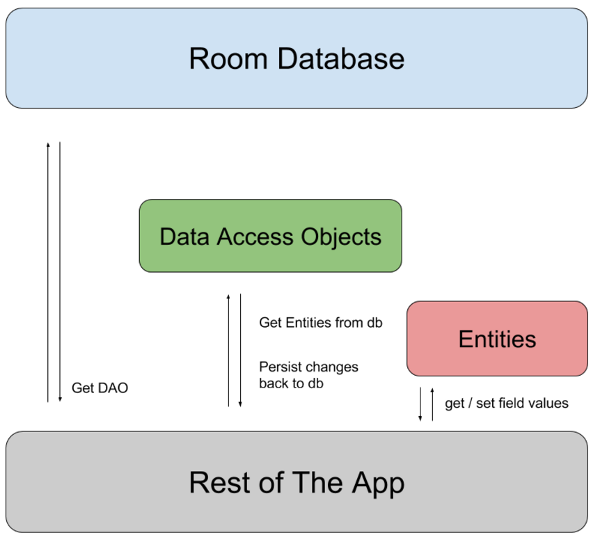
\includegraphics[width = 0.7\textwidth]{figures/room_architecture.png}
	\caption[Room architecture]{Architecture of Android Room database\footnote{https://medium.com/mindorks/using-room-database-android-jetpack-675a89a0e942}}
	\label{fig:room_architecture}
\end{figure}

% 3 richtige quelle https://developer.android.com/training/data-storage/room


\subsubsection{Communication of database and UI}

As the user of our app should always be able to view an up-to-date version of his or her data, we need to make sure that the apps UI (User Interface) state matches the state of the data which is contained in the database. Accordingly, when performing queries, for example when the user is looking at the app screen which shows the blood pressure or weight graphs, the UI should display the currently correct data and update automatically when this data changes. Therefore, so-called observes are used. Anytime the state of an observed object changes, for example if a table in the database is updated, all observers which are bound to that object are notified and hence can take care of adapting the UI. 

For this purpose, we use \textit{LiveData}\footnote{https://developer.android.com/topic/libraries/architecture/livedata} and \textit{ViewModel}\footnote{https://developer.android.com/topic/libraries/architecture/viewmodel} objects, and an additional repository class as this is common best practice to handle the data communication between a Room database and the app's UI. The following explains the different components and how each of them is used. That is also described in Figure \ref{fig:room_livedata}. 

\begin{itemize}
	\item \textbf{LiveData} \\
	When there are changes in the data, the Room library takes care of updating all LiveData objects, which are observable data holders. Also, LiveData objects are lifecycle-aware, which means that they are aware of the current lifecycle status and relevant lifecycle status changes of the corresponding UI class. Consequently, UI components such as Activities or Fragments observe only relevant data and update only if they are currently in an active lifecycle state. 
	
	\item \textbf{ViewModel} \\
	A ViewModel object acts as the communicating element between the database repository and the UI. The ViewModel holds all the data which is relevant for one UI component wrapped in LiveData objects which take care of updating the data if it is necessary, as explained above. Hence, the UI components no longer have to take care of getting the data as the correct data is always stored in the ViewModel. Additionally, ViewModel objects survive configuration changes of UI components like for example device rotation and are therefore able to always provide the UI with the necessary data. 
	
	\item \textbf{Repository} \\
	The repository class provides a clean API for data access and is the single source of truth for all app data. It is used to manage multiple backend data sources, considering our app these are the global database on the server and the local Room database on the phone. The repository defines the logic for deciding whether to use locally stored data or to fetch data from the server. Also, it handles appropriate threading of database access as such operations have to run on separate threads to avoid blocking the main UI thread with for example long-running database queries. 

\end{itemize}

\begin{figure}[htb]
	\centering
	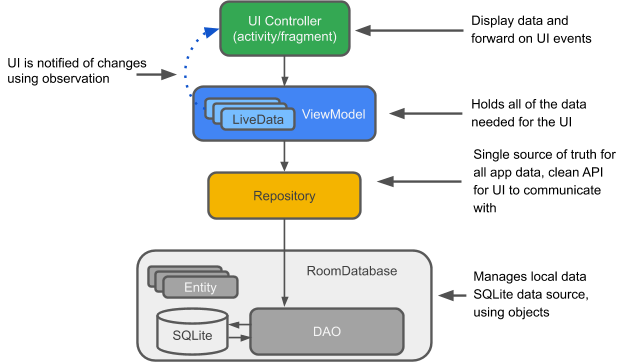
\includegraphics[width = \textwidth]{figures/room_livedata.png}
	\caption[Communication of database and UI]{Communication of database and UI\footnote{https://codelabs.developers.google.com/codelabs/android-room-with-a-view-kotlin}}
	\label{fig:room_livedata}
\end{figure}

In summary, the app uses LiveData objects which take care of observing data changes and updating the currently active UI components with the relevant data if it is necessary. The corresponding data for the UI components is held by ViewModels which are responsible for always providing the up-to-date data to the UI, even during configuration changes. 

There are several advantages of using this combination of architecture components for database-UI-communication. First, manual lifecycle handling it unnecessary and hence, less boilerplate code is needed. In addition, app crashes due to stopped or destroyed Activities and Fragments are avoided as only active UI components are updated. As a result, the UI matches the data status at any time, because all UI components automatically receive the latest data immediately after they come to the foreground and thus are visible for the user \cite{livedata1, livedata2}. 

\subsection{Data synchronization using \textit{Retrofit}}

A major advantage of our system is that the patients' data can be shared with the other types of users, namely next of kin, doctors, and SAPC team members, to ensure that they are always informed about the patient's health status. For example, the SAPC teams can use our web application to monitor the condition of all patients assigned to them. Therefore, synchronization of data between Android devices and our global database on our web server is necessary to make all the needed information available to all different kinds of users of our system. For this purpose, we use the \textit{Retrofit HTTP client}\footnote{https://square.github.io/retrofit/}.

Retrofit is a type-safe HTTP client for Android. The library provides a powerful framework for authenticating and interacting with APIs and sending network requests. Moreover, retrieving and uploading JSON files via a REST-based web service is fairly straightforward. Retrofit maps an HTTP API to a Java interface within our Android app. This is made possible by parsing JSON files, on which the communication with the database located on the webserver is based, into POJOs (Plain Old Java Objects). The resulting POJOs can then be fed into the local Room database \cite{retrofit1, retrofit2}.

To be able to issue network requests to a REST API with Retrofit, API endpoints need to be defined inside of a Java interface. Therefore, Retrofit annotations are used to encode details about the HTTP request method, the parameters, and the method used to dispatch the network call. Also, the relative URL needs to be defined. Examples for such Retrofit annotations are \texttt{@GET} or \texttt{@POST}. This works similar to the mapping of SQL queries to Java function within the DAO interfaces for Room database \cite{retrofit1}. 

Using the Retrofit HTTP client has several advantages compared to developing an own server app communication. It is ideal for use-cases where direct communication with the webserver is intended which is the case for our system. As Retrofit takes care of converting JSON files to POJOs there is no need for manually defining the parsing operation which makes using Retrofit very low effort. Furthermore, Retrofit allows asynchronous handling of server access operations which leads to better app performance as the server access does not block any other operations \cite{retrofit2}.

